\documentclass{beamer}
\usepackage{amsmath,graphics}
\usepackage{amssymb}

\usetheme{default}
\usepackage{xcolor}

\definecolor{solarizedBase03}{HTML}{002B36}
\definecolor{solarizedBase02}{HTML}{073642}
\definecolor{solarizedBase01}{HTML}{586e75}
\definecolor{solarizedBase00}{HTML}{657b83}
\definecolor{solarizedBase0}{HTML}{839496}
\definecolor{solarizedBase1}{HTML}{93a1a1}
\definecolor{solarizedBase2}{HTML}{EEE8D5}
\definecolor{solarizedBase3}{HTML}{FDF6E3}
\definecolor{solarizedYellow}{HTML}{B58900}
\definecolor{solarizedOrange}{HTML}{CB4B16}
\definecolor{solarizedRed}{HTML}{DC322F}
\definecolor{solarizedMagenta}{HTML}{D33682}
\definecolor{solarizedViolet}{HTML}{6C71C4}
%\definecolor{solarizedBlue}{HTML}{268BD2}
\definecolor{solarizedBlue}{HTML}{134676}
\definecolor{solarizedCyan}{HTML}{2AA198}
\definecolor{solarizedGreen}{HTML}{859900}
\definecolor{myBlue}{HTML}{162DB0}%{261CA4}
\setbeamercolor*{item}{fg=myBlue}
\setbeamercolor{normal text}{fg=solarizedBase03, bg=solarizedBase3}
\setbeamercolor{alerted text}{fg=myBlue}
\setbeamercolor{example text}{fg=myBlue, bg=solarizedBase3}
\setbeamercolor*{frametitle}{fg=solarizedRed}
\setbeamercolor*{title}{fg=solarizedRed}
\setbeamercolor{block title}{fg=myBlue, bg=solarizedBase3}
\setbeameroption{hide notes}
\setbeamertemplate{note page}[plain]
\beamertemplatenavigationsymbolsempty
\usefonttheme{professionalfonts}
\usefonttheme{serif}

\usepackage{fourier}

\def\vec#1{\mathchoice{\mbox{\boldmath$\displaystyle#1$}}
{\mbox{\boldmath$\textstyle#1$}}
{\mbox{\boldmath$\scriptstyle#1$}}
{\mbox{\boldmath$\scriptscriptstyle#1$}}}
\definecolor{OwnGrey}{rgb}{0.560,0.000,0.000} % #999999
\definecolor{OwnBlue}{rgb}{0.121,0.398,0.711} % #1f64b0
\definecolor{red4}{rgb}{0.5,0,0}
\definecolor{blue4}{rgb}{0,0,0.5}
\definecolor{Blue}{rgb}{0,0,0.66}
\definecolor{LightBlue}{rgb}{0.9,0.9,1}
\definecolor{Green}{rgb}{0,0.5,0}
\definecolor{LightGreen}{rgb}{0.9,1,0.9}
\definecolor{Red}{rgb}{0.9,0,0}
\definecolor{LightRed}{rgb}{1,0.9,0.9}
\definecolor{White}{gray}{1}
\definecolor{Black}{gray}{0}
\definecolor{LightGray}{gray}{0.8}
\definecolor{Orange}{rgb}{0.1,0.2,1}
\setbeamerfont{sidebar right}{size=\scriptsize}
\setbeamercolor{sidebar right}{fg=Black}

\renewcommand{\emph}[1]{{\textcolor{solarizedRed}{\itshape #1}}}

\newcommand\cA{\mathcal A}
\newcommand\cB{\mathcal B}
\newcommand\cC{\mathcal C}
\newcommand\cD{\mathcal D}
\newcommand\cE{\mathcal E}
\newcommand\cF{\mathcal F}
\newcommand\cG{\mathcal G}
\newcommand\cH{\mathcal H}
\newcommand\cI{\mathcal I}
\newcommand\cJ{\mathcal J}
\newcommand\cK{\mathcal K}
\newcommand\cL{\mathcal L}
\newcommand\cM{\mathcal M}
\newcommand\cN{\mathcal N}
\newcommand\cO{\mathcal O}
\newcommand\cP{\mathcal P}
\newcommand\cQ{\mathcal Q}
\newcommand\cR{\mathcal R}
\newcommand\cS{\mathcal S}
\newcommand\cT{\mathcal T}
\newcommand\cU{\mathcal U}
\newcommand\cV{\mathcal V}
\newcommand\cW{\mathcal W}
\newcommand\cX{\mathcal X}
\newcommand\cY{\mathcal Y}
\newcommand\cZ{\mathcal Z}

\newcommand\fA{\mathfrak A}
\newcommand\fB{\mathfrak B}
\newcommand\fC{\mathfrak C}
\newcommand\fD{\mathfrak D}
\newcommand\fE{\mathfrak E}
\newcommand\fF{\mathfrak F}
\newcommand\fG{\mathfrak G}
\newcommand\fH{\mathfrak H}
\newcommand\fI{\mathfrak I}
\newcommand\fJ{\mathfrak J}
\newcommand\fK{\mathfrak K}
\newcommand\fL{\mathfrak L}
\newcommand\fM{\mathfrak M}
\newcommand\fN{\mathfrak N}
\newcommand\fO{\mathfrak O}
\newcommand\fP{\mathfrak P}
\newcommand\fQ{\mathfrak Q}
\newcommand\fR{\mathfrak R}
\newcommand\fS{\mathfrak S}
\newcommand\fT{\mathfrak T}
\newcommand\fU{\mathfrak U}
\newcommand\fV{\mathfrak V}
\newcommand\fW{\mathfrak W}
\newcommand\fX{\mathfrak X}
\newcommand\fY{\mathfrak Y}
\newcommand\fZ{\mathfrak Z}

\newcommand\fa{\mathfrak a}
\newcommand\fb{\mathfrak b}
\newcommand\fc{\mathfrak c}
\newcommand\fd{\mathfrak d}
\newcommand\fe{\mathfrak e}
\newcommand\ff{\mathfrak f}
\newcommand\fg{\mathfrak g}
\newcommand\fh{\mathfrak h}
%\newcommand\fi{\mathfrak i}
\newcommand\fj{\mathfrak j}
\newcommand\fk{\mathfrak k}
\newcommand\fl{\mathfrak l}
\newcommand\fm{\mathfrak m}
\newcommand\fn{\mathfrak n}
\newcommand\fo{\mathfrak o}
\newcommand\fp{\mathfrak p}
\newcommand\fq{\mathfrak q}
\newcommand\fr{\mathfrak r}
\newcommand\fs{\mathfrak s}
\newcommand\ft{\mathfrak t}
\newcommand\fu{\mathfrak u}
\newcommand\fv{\mathfrak v}
\newcommand\fw{\mathfrak w}
\newcommand\fx{\mathfrak x}
\newcommand\fy{\mathfrak y}
\newcommand\fz{\mathfrak z}

\newcommand\vA{\vec A}
\newcommand\vB{\vec B}
\newcommand\vC{\vec C}
\newcommand\vD{\vec D}
\newcommand\vE{\vec E}
\newcommand\vF{\vec F}
\newcommand\vG{\vec G}
\newcommand\vH{\vec H}
\newcommand\vI{\vec I}
\newcommand\vJ{\vec J}
\newcommand\vK{\vec K}
\newcommand\vL{\vec L}
\newcommand\vM{\vec M}
\newcommand\vN{\vec N}
\newcommand\vO{\vec O}
\newcommand\vP{\vec P}
\newcommand\vQ{\vec Q}
\newcommand\vR{\vec R}
\newcommand\vS{\vec S}
\newcommand\vT{\vec T}
\newcommand\vU{\vec U}
\newcommand\vV{\vec V}
\newcommand\vW{\vec W}
\newcommand\vX{\vec X}
\newcommand\vY{\vec Y}
\newcommand\vZ{\vec Z}

\newcommand\va{\vec a}
\newcommand\vb{\vec b}
\newcommand\vc{\vec c}
\newcommand\vd{\vec d}
\newcommand\ve{\vec e}
\newcommand\vf{\vec f}
\newcommand\vg{\vec g}
\newcommand\vh{\vec h}
\newcommand\vi{\vec i}
\newcommand\vj{\vec j}
\newcommand\vk{\vec k}
\newcommand\vl{\vec l}
\newcommand\vm{\vec m}
\newcommand\vn{\vec n}
\newcommand\vo{\vec o}
\newcommand\vp{\vec p}
\newcommand\vq{\vec q}
\newcommand\vr{\vec r}
\newcommand\vs{\vec s}
\newcommand\vt{\vec t}
\newcommand\vu{\vec u}
\newcommand\vv{\vec v}
\newcommand\vw{\vec w}
\newcommand\vx{\vec x}
\newcommand\vy{\vec y}
\newcommand\vz{\vec z}

\renewcommand\AA{\mathbb A}
\newcommand\NN{\mathbb N}
\newcommand\ZZ{\mathbb Z}
\newcommand\PP{\mathbb P}
\newcommand\QQ{\mathbb Q}
\newcommand\RR{\mathbb R}
\renewcommand\SS{\mathbb S}
\newcommand\CC{\mathbb C}

\newcommand{\ord}{\mathrm{ord}}
\newcommand{\id}{\mathrm{id}}
\newcommand{\pr}{\mathrm{P}}
\newcommand{\Vol}{\mathrm{vol}}
\newcommand\norm[1]{\left\|{#1}\right\|} 
\newcommand\sign{\mathrm{sign}}
\newcommand{\eps}{\varepsilon}
\newcommand{\abs}[1]{\left|#1\right|}
\newcommand\bc[1]{\left({#1}\right)} 
\newcommand\cbc[1]{\left\{{#1}\right\}} 
\newcommand\bcfr[2]{\bc{\frac{#1}{#2}}} 
\newcommand{\bck}[1]{\left\langle{#1}\right\rangle} 
\newcommand\brk[1]{\left\lbrack{#1}\right\rbrack} 
\newcommand\scal[2]{\bck{{#1},{#2}}} 
\newcommand{\vecone}{\mathbb{1}}
\newcommand{\tensor}{\otimes}
\newcommand{\diag}{\mathrm{diag}}
\newcommand{\ggt}{\mathrm{ggT}}
\newcommand{\kgv}{\mathrm{kgV}}

\newcommand{\Karonski}{Karo\'nski}
\newcommand{\Erdos}{Erd\H{o}s}
\newcommand{\Renyi}{R\'enyi}
\newcommand{\Lovasz}{Lov\'asz}
\newcommand{\Juhasz}{Juh\'asz}
\newcommand{\Bollobas}{Bollob\'as}
\newcommand{\Furedi}{F\"uredi}
\newcommand{\Komlos}{Koml\'os}
\newcommand{\Luczak}{\L uczak}
\newcommand{\Kucera}{Ku\v{c}era}
\newcommand{\Szemeredi}{Szemer\'edi}

\renewcommand{\ae}{\"a}
\renewcommand{\oe}{\"o}
\newcommand{\ue}{\"u}
\newcommand{\Ae}{\"A}
\newcommand{\Oe}{\"O}
\newcommand{\Ue}{\"U}

\title[Linadi]{Gruppen}
\author[Amin Coja-Oghlan]{Amin Coja-Oghlan}
\institute[Frankfurt]{JWGUFFM}
\date{}

\begin{document}

\frame[plain]{\titlepage}

\begin{frame}\frametitle{Gruppen}
	\begin{block}{Definition}
		Eine \emph{Gruppe} ist eine Menge $G$ zusammen mit einer Abbildung 
		\begin{align*}
			*:G\times G\to G,&&(x,y)\mapsto x*y
		\end{align*}
 die folgende Bedingungen erf\"ullt:
		\begin{description}
			\item[Assoziativgesetz:] f\ue r alle $x,y,z\in G$ gilt $$(x*y)*z=x*(y*z).$$
			\item[Neutrales Element:] es gibt ein $e\in G$, so da\ss\ f\ue r alle $x\in G$ gilt $$e*x=x.$$
			\item[Inverses Element:] zu jedem $x\in G$ gibt es ein $y\in G$ mit $$y*x=e.$$
		\end{description}
	\end{block}
\end{frame}

\begin{frame}\frametitle{Gruppen}
	\begin{overprint}
		\onslide<1>	
		\begin{block}{Beispiel}
			\begin{itemize}
				\item $G=\ZZ$, $*=+$
				\item Zahlenbeispiel f\ue r die Verkn\ue pfung:
					\begin{align*}
						7+5&=12&&7+(-5)=2
					\end{align*}
				\item Das neutrale Element ist $0$.
				\item Das Inverse zu $x\in\ZZ$ ist die Zahl $-x$.
				\item Beispielsweise ist $-7$ das Inverse zu $7$.
				\item {\itshape Was ist das Inverse zu $0$?}
			\end{itemize}
		\end{block}	
		\onslide<2>	
		\begin{block}{Beispiel}
			\begin{itemize}
				\item $G=\QQ\setminus\cbc0$, $*=\,\cdot\,$
				\item Zahlenbeispiel f\ue r die Verkn\ue pfung:
					\begin{align*}
						\frac{7}{5}\cdot\frac{-2}{3}&=\frac{-14}{15}&&\frac{11}{7}\cdot\frac{7}{11}&=\frac{1}{1}
					\end{align*}
				\item Das neutrale Element ist $1=\frac{1}{1}$.
				\item Das Inverse zu $\frac{x}{y}\in\QQ\setminus\cbc0$ ist die Zahl $\frac{y}{x}$.
				\item Beispielsweise ist $\frac{11}{7}$ das Inverse zu $\frac{7}{11}$.
			\end{itemize}
		\end{block}	
		\onslide<3>
		\begin{block}{Beispiel}
			\begin{itemize}
				\item Die \alert{Kleinsche Vierergruppe} besteht aus $G=\{e,a,b,c\}$ und der Verkn\ue pfung $*$, die durch folgende Tabelle definiert ist:
					\begin{center}
						\begin{tabular}{c|cccc}
							*&e&a&b&c\\\hline
							e&e&a&b&c\\
							a&a&e&c&b\\
							b&b&c&e&a\\
							c&c&b&a&e
						\end{tabular}
					\end{center}
				\item Konkrete Beispiele f\ue r die Verkn\ue pfung:
					\begin{align*}
						a*b&=c&&a*a=e&&c*b=a
					\end{align*}
				\item F\ue r alle Element $x\in G$ gilt $x^{-1}=x$.
			\end{itemize}		
		\end{block}
		\onslide<4>
		\begin{block}{Beispiel}
			\begin{itemize}
				\item Die \alert{symmetrische Gruppe} $\SS_n$ besteht aus allen bijektiven Abbildungen $\{1,2,3,\ldots,n\}\to\{1,2,3,\ldots,n\}$.
				\item Diese Abbildungen werden auch \emph{Permutationen} genannt.
				\item Die Verkn\ue pfung $*$ ist die Komposition $\circ$ von Abbildungen.
				\item F\ue r $\sigma,\tau\in\SS_n$ ist
					\begin{align*}
						\sigma\circ\tau:\{1,2,3,\ldots,n\}&\to\{1,2,3,\ldots,n\},\qquad k\mapsto\sigma(\tau(k)).
					\end{align*}
				\item Das neutrale Element ist 
					\begin{align*}
						\id&:\{1,2,3,\ldots,n\}\to\{1,2,3,\ldots,n\},&k\mapsto k.
					\end{align*}
				\item Das Inverse zu $\sigma\in\SS_n$ ist die Umkehrabbildung $\sigma^{-1}$.
			\end{itemize}	
		\end{block}
		\onslide<5>
		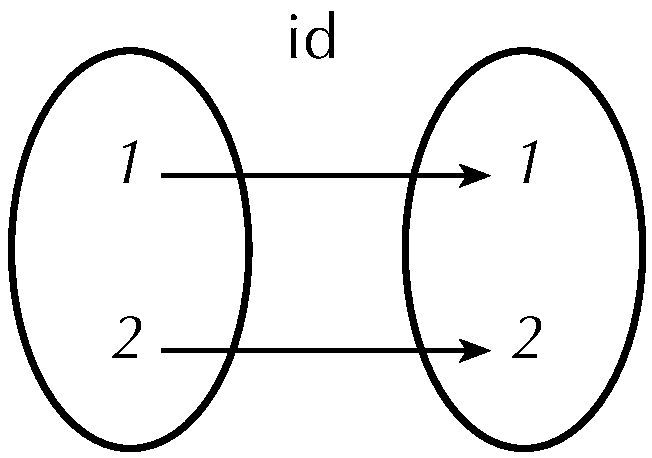
\includegraphics[height=20mm]{pics/id.pdf}\hfill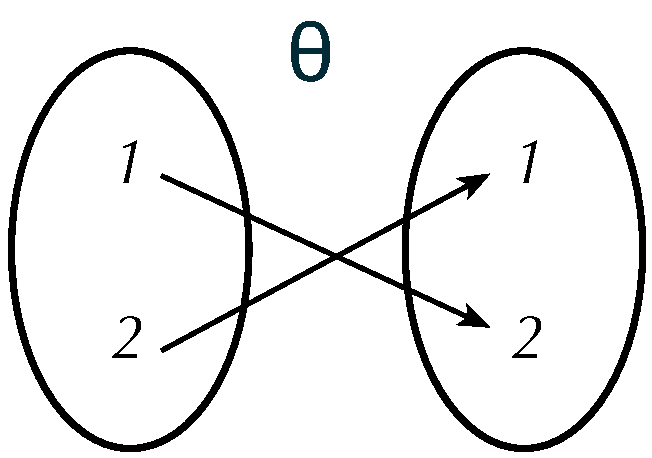
\includegraphics[height=20mm]{pics/theta.pdf}
		\begin{block}{Beispiel}
			\begin{itemize}
				\item Konkret besteht $\SS_2$ aus zwei Abbildungen $\{1,2\}\to\{1,2\}$:
					\begin{align*}
						\id:1&\mapsto1&2\mapsto2\\
						\theta:1&\mapsto2&2\mapsto1
					\end{align*}
			\end{itemize}	
		\end{block}
		\onslide<6>
		\hfill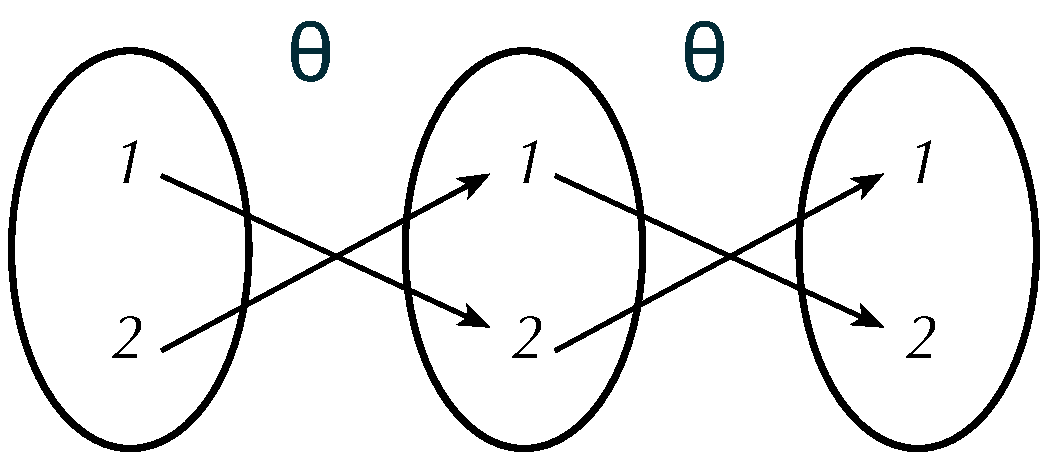
\includegraphics[height=20mm]{pics/thetatheta.pdf}
		\begin{block}{Beispiel}
			\begin{itemize}
			\item Beispielverkn\ue pfung $\theta\circ\theta$:
					\begin{align*}
						\theta\circ\theta(1)&=\theta(\theta(1))=\theta(2)=1\\
						\theta\circ\theta(2)&=\theta(\theta(2))=\theta(1)=2
					\end{align*}
				\item Verkn\ue pfungstabelle:
					\begin{align*}
						\begin{array}{c|c|c}
							\circ&\id&\theta\\\hline
							\id&\id&\theta\\\hline
							\theta&\theta&\id
						\end{array}
					\end{align*}
			\end{itemize}	
		\end{block}
	\end{overprint}
\end{frame}

\begin{frame}\frametitle{Gruppen}
	\begin{block}{Lemma}
		Sei $(G,*)$ eine Gruppe.
		\begin{enumerate}
			\item Es gibt genau ein neutrales Element $e$.
			\item Dieses erf\ue llt $x*e=x$ f\ue r alle $x\in G$.
			\item Zu jedem $x\in G$ gibt es genau ein Inverses $x^{*-1}$.
			\item Dieses erf\ue llt $x*x^{*-1}=e$.
		\end{enumerate}
	\end{block}
	\begin{overprint}
		\onslide<1>
		\begin{block}{Beweis}
			\begin{itemize}
				\item \alert{zu 4.:} angenommen $y*x=e$; sei $z$ invers zu $y$, d.h.\ $z*y=e$. \item Folglich
					\begin{align*}
						x*y&=e*(x*y)=(z*y)*(x*y)=(z*(y*x))*y\\&=(z*e)*y=z*(e*y)=z*y=e.
					\end{align*}
			\end{itemize}
		\end{block}	
		\onslide<2>
		\begin{block}{Beweis (Fortsetzung)}
			\begin{itemize}
				\item \alert{zu 2.:} angenommen $e$ ist neutral.
				\item  Sei $x\in G$ und $y$ invers zu $x$.
				\item Nach 4.\ gilt
					\begin{align*}
						x*e=x*(y*x)=(x*y)*x=e*x=x.
					\end{align*}
			\end{itemize}	
		\end{block}
		\onslide<3>
		\begin{block}{Beweis (Fortsetzung)}
			\begin{itemize}
				\item \alert{zu 1.:} angenommen $e,f$ sind neutral.
				\item Nach 2.\ gilt
					\begin{align*}
						f=e*f=e.
					\end{align*}
			\end{itemize}	
		\end{block}
		\onslide<4>
		\begin{block}{Beweis (Fortsetzung)}
			\begin{itemize}
				\item \alert{zu 3.:} angenommen $y,z$ sind invers zu $x$.
				\item Nach 2.\ und 4.\ gilt
					\begin{align*}
						y=y*e=y*(x*z)=(y*x)*z=e*z=z.
					\end{align*}
			\end{itemize}	
		\end{block}
	\end{overprint}
\end{frame}

\begin{frame}\frametitle{Gruppen}
	\begin{block}{Lemma}
		Sei $(G,*)$ eine Gruppe und seien $x,y\in G$.
		\begin{enumerate}
			\item Es gilt $(x^{*-1})^{*-1}=x$.
			\item Es gilt $(x*y)^{*-1}=y^{*-1}*x^{*-1}$.
		\end{enumerate}
	\end{block}
	\begin{block}{Beweis}
		\begin{itemize}
			\item \alert{zu 1.:} wir haben $x*x^{*-1}=e$ nach dem vorherigen Lemma.
			\item \alert{zu 2.:} es gilt
				\begin{align*}
					(y^{*-1}*x^{*-1})*(x*y)&=y^{*-1}*((x^{*-1}*x)*y)=y^{*-1}*(e*y)\\&=y^{*-1}*y=e.
				\end{align*} 
		\end{itemize}
	\end{block}
\end{frame}

\begin{frame}\frametitle{Gruppen}
	\begin{block}{Schreibweise}
		\begin{itemize}
			\item Sei $(G,*)$ eine Gruppe.
			\item Zu $x\in G$ und $\ell\in\NN$ bezeichnet
				\begin{align*}
					x^{*\ell}=\underbrace{x*\cdots*x}_{\mbox{$\ell$ mal}}.
				\end{align*}
			\item Zu $x\in G$ und $\ell\in\NN$ bezeichnet
				\begin{align*}
					x^{*-\ell}=\underbrace{x^{*-1}*\cdots*x^{*-1}}_{\mbox{$\ell$ mal}}.
				\end{align*}
			\item Zu $x\in G$ ist $x^{*0}=e$ das neutrale Element.
		\end{itemize}
	\end{block}
\end{frame}


\begin{frame}\frametitle{Homomorphismen}
	\begin{block}{Definition}
		\begin{itemize}
			\item Seien $(G,*),(H,\star)$ zwei Gruppen.
			\item Eine Abbildung $f:G\to H$ hei\ss t \emph{Homomorphismus} falls 
				\begin{align*}
					f(x*y)=f(x)\star f(y)&&\mbox{f\ue r alle }x,y\in G.
				\end{align*}
		\end{itemize}
	\end{block}
\end{frame}

\begin{frame}\frametitle{Homomorphismen}
	\begin{block}{Beispiel}
		\begin{itemize}
			\item Seien $(G,*)=(H,\star)=(\ZZ,+)$.
			\item Die Abbildung $f:\ZZ\to\ZZ$, $x\mapsto -x$ ist ein Homomorphismus.
			\item Denn $f(x+y)=-(x+y)=-x+(-y)=f(x)+f(y)$.
		\end{itemize}
	\end{block}
\end{frame}

\begin{frame}\frametitle{Homomorphismen}
	\begin{block}{Beispiel}
		\begin{itemize}
			\item Seien $(G,*)=(\ZZ,+)$ und $(H,\star)=(\QQ\cbc0,\,\cdot\,)$.
			\item Die Abbildung $f:\ZZ\to\QQ\cbc0$, $x\mapsto 2^x$ ist ein Homomorphismus.
			\item Denn 
				\begin{align*}
					f(x+y)=2^{x+y}=2^x\cdot 2^y=f(x)\cdot f(y).
				\end{align*}
		\end{itemize}
	\end{block}
\end{frame}

\begin{frame}\frametitle{Homomorphismen}
	\begin{block}{Beispiel}
		\begin{itemize}
			\item Seien $(G,*)=(H,\star)=(\SS_n,\circ)$.
			\item Sei $\gamma\in\SS_n$ irgendeine bestimmte Permutation.
			\item Dann ist die Abbildung
				\begin{align*}
					f:\SS_n\to\SS_n,\qquad \sigma\mapsto \gamma^{-1}\circ\sigma\circ\gamma
				\end{align*}
				ein Homomorphismus.
			\item Denn
				\begin{align*}
					f(\sigma\circ\tau)=\gamma^{-1}\circ\sigma\circ\tau\circ\gamma=\gamma^{-1}\circ\sigma\circ\gamma\circ\gamma^{-1}\circ\tau\circ\gamma=f(\sigma)\circ f(\tau).
				\end{align*}
		\end{itemize}
	\end{block}
\end{frame}

\begin{frame}\frametitle{Untergruppen}
	\begin{block}{Definition}
		\begin{itemize}
			\item Sei $(G,*)$ eine Gruppe.
			\item Eine Teilmenge $H\subseteq G$ hei\ss t \emph{Untergruppe} von $G$, wenn $H\neq\emptyset$ und
				\begin{align*}
					x^{*-1}*y&\in H&&\mbox{f\ue r alle }x,y\in H.
				\end{align*}
		\end{itemize}
	\end{block}
	\begin{block}{Bemerkung}
		Eine Untergruppe $H$ von $G$ ist mit der Verkn\ue pfung $*$ selbst eine Gruppe.
	\end{block}
\end{frame}

\begin{frame}\frametitle{Untergruppen}
	\begin{overprint}
		\onslide<1>
		\begin{block}{Beispiel}
			\begin{itemize}
				\item Die Menge aller durch 5 teilbaren Zahlen, also
					\begin{align*}
						H=5\cdot\ZZ=\cbc{5\cdot z:z\in\ZZ}
					\end{align*}
					ist eine Untergruppe von $(\ZZ,+)$.
				\item Denn wenn $x,y\in H$, dann gilt $5\mid x$ und $5\mid y$, also auch
					\begin{align*}
						5\mid -x+y=y-x,
					\end{align*}
					weshalb $-x+y\in H$.
				\item Allgemeiner ist f\ue r jedes $n\in\ZZ$ die Menge $ n\cdot\ZZ=\{n\cdot z:z\in\ZZ\} $ aller Vielfachen von $n$ eine Untergruppe.
				\item Die Mengen $n\cdot\ZZ$ weren \emph{arithmetische Progressionen} genannt.
			\end{itemize}
		\end{block}
		\onslide<2>
		\begin{block}{Beispiel}
			\begin{itemize}
				\item Die Menge aller Potenzen von zwei, also
					\begin{align*}
						H&=\cbc{2^a:a\in\ZZ}
					\end{align*}
					ist eine Untergruppe von $(\QQ\cbc0,\,\cdot\,)$.
				\item Denn wenn $x=2^a,y=2^b\in H$, dann gilt auch
					\begin{align*}
						x^{-1}\cdot y=2^{-a}\cdot 2^b=2^{-a+b}\in H.
					\end{align*}
			\end{itemize}
		\end{block}
	\end{overprint}
\end{frame}

\begin{frame}\frametitle{Untergruppen}
	\begin{block}{Definition}
		\begin{itemize}
			\item Sei $(G,*)$ eine Gruppe und $H$ eine Untergruppe.
			\item die Mengen $$x*H=\{x*y:y\in H\}$$ hei\ss en \emph{Linksnebenklassen} von $H$ in $G$.
			\item die Mengen $$H*x=\{y*x:y\in H\}$$ hei\ss en \emph{Rechtsnebenklassen} von $H$ in $G$.
		\end{itemize}
	\end{block}	
\end{frame}

\begin{frame}\frametitle{Untergruppen}
	\begin{block}{Lemma}
		Sei $(G,*)$ eine Gruppe und $H$ eine Untergruppe.
		\begin{itemize}
			\item Zwei Linksnebenklassen $x*H$, $x'*H$ sind entweder gleich oder disjunkt.
			\item Es gilt $|x*H|=|H|$.
		\end{itemize}
	\end{block}	
	\begin{overprint}
		\onslide<1>
		\begin{block}{Beweis}
			\begin{itemize}
				\item Angenommen $(x*H)\cap(x'*H)\neq\emptyset$.
				\item Dann gibt es $z,z'\in G$ mit $x*z=x'*z'$.
				\item F\ue r jedes $y\in G$ gilt also
					\begin{align*}
						x*y=x*z*z^{*-1}*y=x'*z'*z^{*-1}*y\in x'*H.
					\end{align*}
				\item Also $x*H\subseteq x'*H$.
				\item Analog sieht man $x'*H\subseteq x*H$.
			\end{itemize}	
		\end{block}	
		\onslide<2>
		\begin{block}{Beweis (Fortsetzung)}
			\begin{itemize}
				\item Definiere eine Abbildung $H\to x*H$, $y\mapsto x*y$.
				\item Diese Abbildung ist surjektiv.
				\item Sie ist auch injektiv, denn 
					\begin{align*}
						x*y=x*y'\quad\Rightarrow\quad x^{*-1}*x*y=x^{*-1}*x*y'\quad\Rightarrow\quad y=y'.
					\end{align*}
				\item Also ist die Abbildung bijektiv und $|x*H|=|H|$.
			\end{itemize}	
		\end{block}
	\end{overprint}
\end{frame}

\begin{frame}\frametitle{Untergruppen}
	\begin{block}{Satz von Lagrange}
		Sei $(G,*)$ eine endliche Gruppe und $H$ eine Untergruppe.
		Sei
		\begin{align*}
			|G:H|=\abs{\cbc{x*H:x\in G}}
		\end{align*}
		die Anzahl verschiedener Linksnebenklassen.
		Dann gilt $$|G|=|H|\cdot|G:H|$$ und insbesondere $|H|\mid|G|$.
	\end{block}
	\begin{block}{Beweis}
		Unmittelbare Konsequenz des Lemmas.
	\end{block}
\end{frame}

\begin{frame}\frametitle{Die Ordnung}
	\begin{block}{Definition}
		Die \emph{Ordnung} eines Elements $x$ einer Gruppe $(G,*)$ ist
		\begin{align*}
			\ord_G(x)&=\min\cbc{\ell\in\NN:x^{*\ell}=e}.
		\end{align*}
	\end{block}
	\begin{block}{Anmerkung}
		\begin{itemize}
			\item $\ord_G(x)\in\NN\cup\cbc\infty$.
			\item $\ord_G(x)\leq|G|$.
			\item $\ord_G(x)=\ord_G(x^{*-1})$.
		\end{itemize}
	\end{block}
\end{frame}

\begin{frame}\frametitle{Die Ordnung}
	\begin{block}{Proposition}
		Sei $(G,*)$ eine endliche Gruppe und $x\in G$.
		Dann gilt $\ord_G(x)\mid|G|$.
	\end{block}
	\begin{block}{Beweis}
		\begin{itemize}
			\item Die Menge $\bck x=\{x^{*\ell}:\ell\geq0\}$ ist eine Untergruppe.
			\item Denn wenn $\ell=\ord_G(x)$, gilt $x^{*-1}=x^{*\ell-1}\in\bck x$.
			\item Es gilt $|\bck x|=\ord_G(x)$.
			\item Also folgt die Behauptung aus dem Satz von Lagrange.
		\end{itemize}
	\end{block}
\end{frame}

\begin{frame}\frametitle{Die Ordnung}
	\begin{block}{Satz (``Kleiner Fermat'')}
		Sei $(G,*)$ eine endliche Gruppe und $x\in G$.
		Dann gilt $$x^{*|G|}=e.$$
	\end{block}
	\begin{block}{Beweis}
	Wir schreiben	
	\begin{align*}
		x^{*|G|}=\bc{x^{*\ord_G(x)}}^{*|G|/\ord_G(x)}=e^{*|G|/\ord_G(x)}=e.
	\end{align*}
	\end{block}
\end{frame}

\begin{frame}\frametitle{Beispiele}
	\begin{overprint}
		\onslide<1>	
		\begin{block}{Beispiel}
			\begin{itemize}
				\item $G=\ZZ$, $*=+$
				\item Es gilt $\ord_{\ZZ}0=1$.
				\item Es gilt $\ord_{\ZZ}z=\infty$ f\ue r alle $z\neq0$.
			\end{itemize}
		\end{block}	
		\onslide<2>	
		\begin{block}{Beispiel}
			\begin{itemize}
				\item $G=\QQ\setminus\cbc0$, $*=\,\cdot\,$
				\item Es gilt $\ord_{\QQ\setminus\cbc0}1=1$.
				\item Es gilt $\ord_{\QQ\setminus\cbc0}z=\infty$ f\ue r alle $z\neq1$.
			\end{itemize}
		\end{block}	
		\onslide<3>
		\begin{block}{Beispiel}
			\begin{itemize}
				\item Die Kleinsche Vierergruppe $K$:
					\begin{center}
						\begin{tabular}{c|cccc}
							*&e&a&b&c\\\hline
							e&e&a&b&c\\
							a&a&e&c&b\\
							b&b&c&e&a\\
							c&c&b&a&e
						\end{tabular}
					\end{center}
				\item Wie in jeder Gruppe gilt $\ord_Ke=1$.
				\item Es gilt $\ord_Ka=\ord_Kb=\ord_Kc=2$, denn
					\begin{align*}
					a*a=b*b=c*c=e.
					\end{align*}
				\item $\bck a=\{e,a\}$
			\end{itemize}		
		\end{block}
		\onslide<4>
			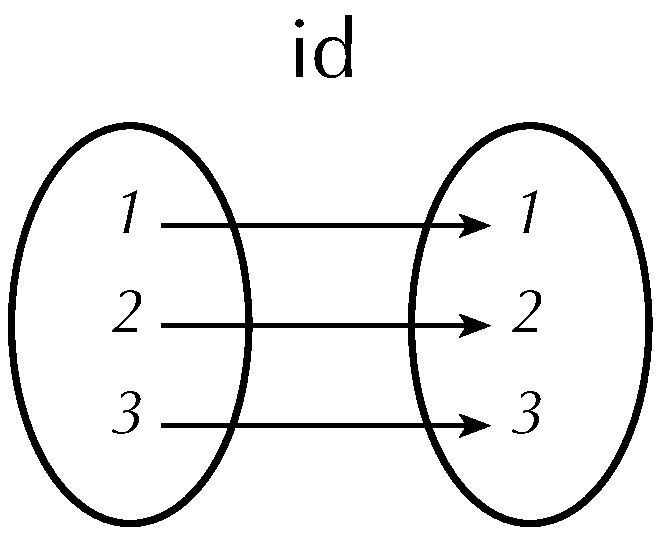
\includegraphics[height=20mm]{pics/idS3.pdf}\hfill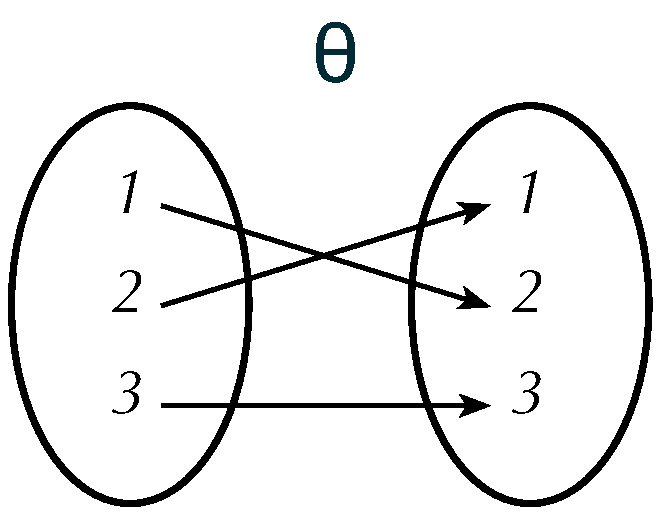
\includegraphics[height=20mm]{pics/thetaS3.pdf}\hfill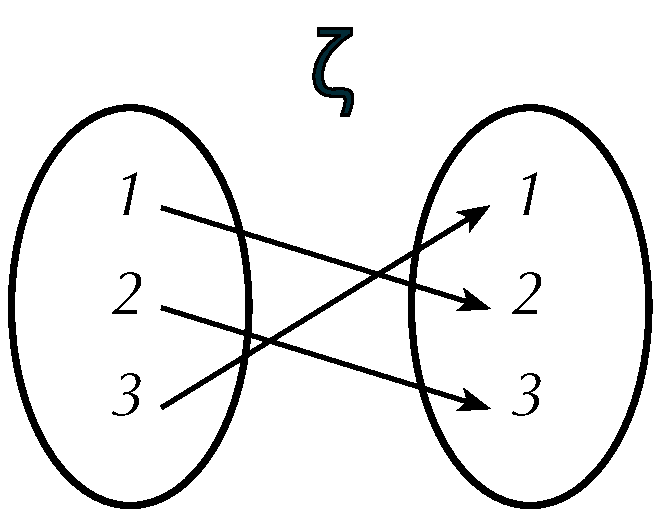
\includegraphics[height=20mm]{pics/zetaS3.pdf}
		\begin{block}{Beispiel}
			\begin{itemize}
				\item Symmetrische Gruppe $\SS_3$ aller Permutation $\{1,2,3\}\to\{1,2,3\}$
				\item Neutrales Element ist die identische Abbildung
					\begin{align*}
					\id:1\mapsto 1,\ 2\mapsto2,\ 3\mapsto3
					\end{align*}
				\item Die Transposition $\theta: 1\mapsto 2,\ 2\mapsto 1,\, 3\mapsto 3 $
					hat Ordnung $2$
				\item Der Zykel $ \zeta:1\mapsto 2,\ 2\mapsto 3,\ 3\mapsto 1 $
					erf\ue llt
					\begin{align*}
					\zeta^2:1\mapsto 3,\ 2\mapsto 1,\ 3\mapsto 2,\qquad \zeta^3=\id
					\end{align*}
					und hat also Ordnung 3.
%				\item Warum gibt es kein Element der Ordnung $6=|\SS_3|$?
			\end{itemize}	
		\end{block}
		\onslide<5>
			\hfill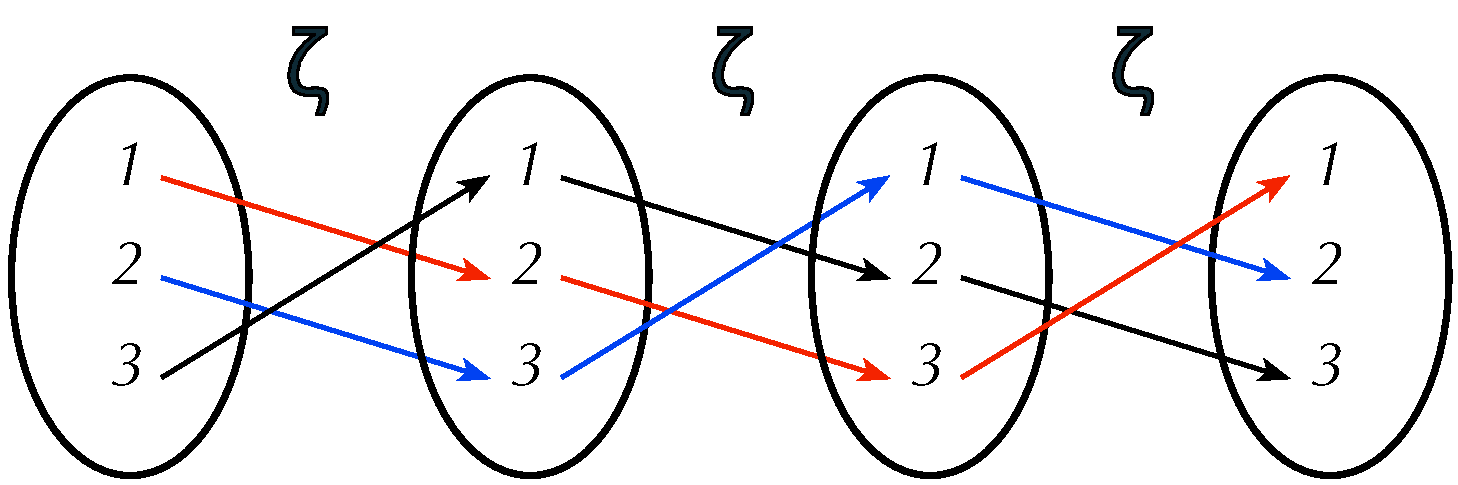
\includegraphics[height=20mm]{pics/zeta3S3.pdf}
		\begin{block}{Beispiel}
			\begin{itemize}
				\item Symmetrische Gruppe $\SS_3$ aller Permutation $\{1,2,3\}\to\{1,2,3\}$
				\item Neutrales Element ist die identische Abbildung
					\begin{align*}
					\id:1\mapsto 1,\ 2\mapsto2,\ 3\mapsto3
					\end{align*}
				\item Die Transposition $\theta: 1\mapsto 2,\ 2\mapsto 1,\, 3\mapsto 3 $
					hat Ordnung $2$
				\item Der Zykel $ \zeta:1\mapsto 2,\ 2\mapsto 3,\ 3\mapsto 1 $
					erf\ue llt
					\begin{align*}
					\zeta^2:1\mapsto 3,\ 2\mapsto 1,\ 3\mapsto 2,\qquad \zeta^3=\id
					\end{align*}
					und hat also Ordnung 3.
%				\item Warum gibt es kein Element der Ordnung $6=|\SS_3|$?
			\end{itemize}	
		\end{block}
	\end{overprint}
\end{frame}

\begin{frame}\frametitle{Zusammenfassung}
\begin{itemize}
\item Der allgemeine Gruppenbegriff
\item Homomorphismen 
\item Ordnungsbegriff
\item Satz von Lagrange
\end{itemize}
\end{frame}

\end{document}
